\section{Data Description}

\subsection{Data Collection}

The data used in this program is provided by Dr. Ciborowski, collected and 
processed by Zhang.
It consists of data from
three separate surveys conducted in: 1991, 1999 and 2004 (Zhang \cite{Zhang2008}; Farara and Burt 1993 \cite{Farara1993}; Wood 2004 \cite{Wood2004}),
all following the same field protocols
\footnote{
These sampling locations were determined prior to 
fieldwork by a stratified random sampling design to ensure representative coverage.}.

The 2004 data set was collected by Zhang \cite{Zhang2008} and principally across the entire SCDRS zone.
The information collected includes sample location information (longitude and latitude),
16 zoobenthic taxonomic variables, 5 environmental
variables (e.g., temperature, pH, dissolved oxygen), and 30 stressors representing trace metals,
polyaromatic hydrocarbons (PAHs).
The data from two previous studies, which collected data from the Detroit River zone in 1991 and 1999
(Farara and Burt 1993 \cite{Farara1993}; Wood 2004 \cite{Wood2004})—were compiled and incorporated into the 2004 data.
This combination enhances the dataset's robustness by providing a more comprehensive perspective on
the benthic community dynamics, environmental conditions, and sediment contamination across the entire Corridor over time.


Given the temporal and spatial distribution of sampling across three survey years,
\textbf{StationID serves as the primary key for data integration and site identification.}
{Each StationID uniquely identifies a sampling site in both temporal and spatial dimensions, 
meaning observations with the same StationID represent identical location-time combinations 
from the three survey years (1991, 1999, 2004).}

\subsection{Prepare a complete sub-dataset for preliminary analysis}

Taxonomic, environmental, and stressor data for sampled sites were originally stored in three separate tabular files.
For preliminary analysis, we made a quick check on the data quality and completeness
\footnote{By the submission 
of the proposal the latest check was done on July 24, 2025.}.

\begin{figure}[!h]
    \centering
    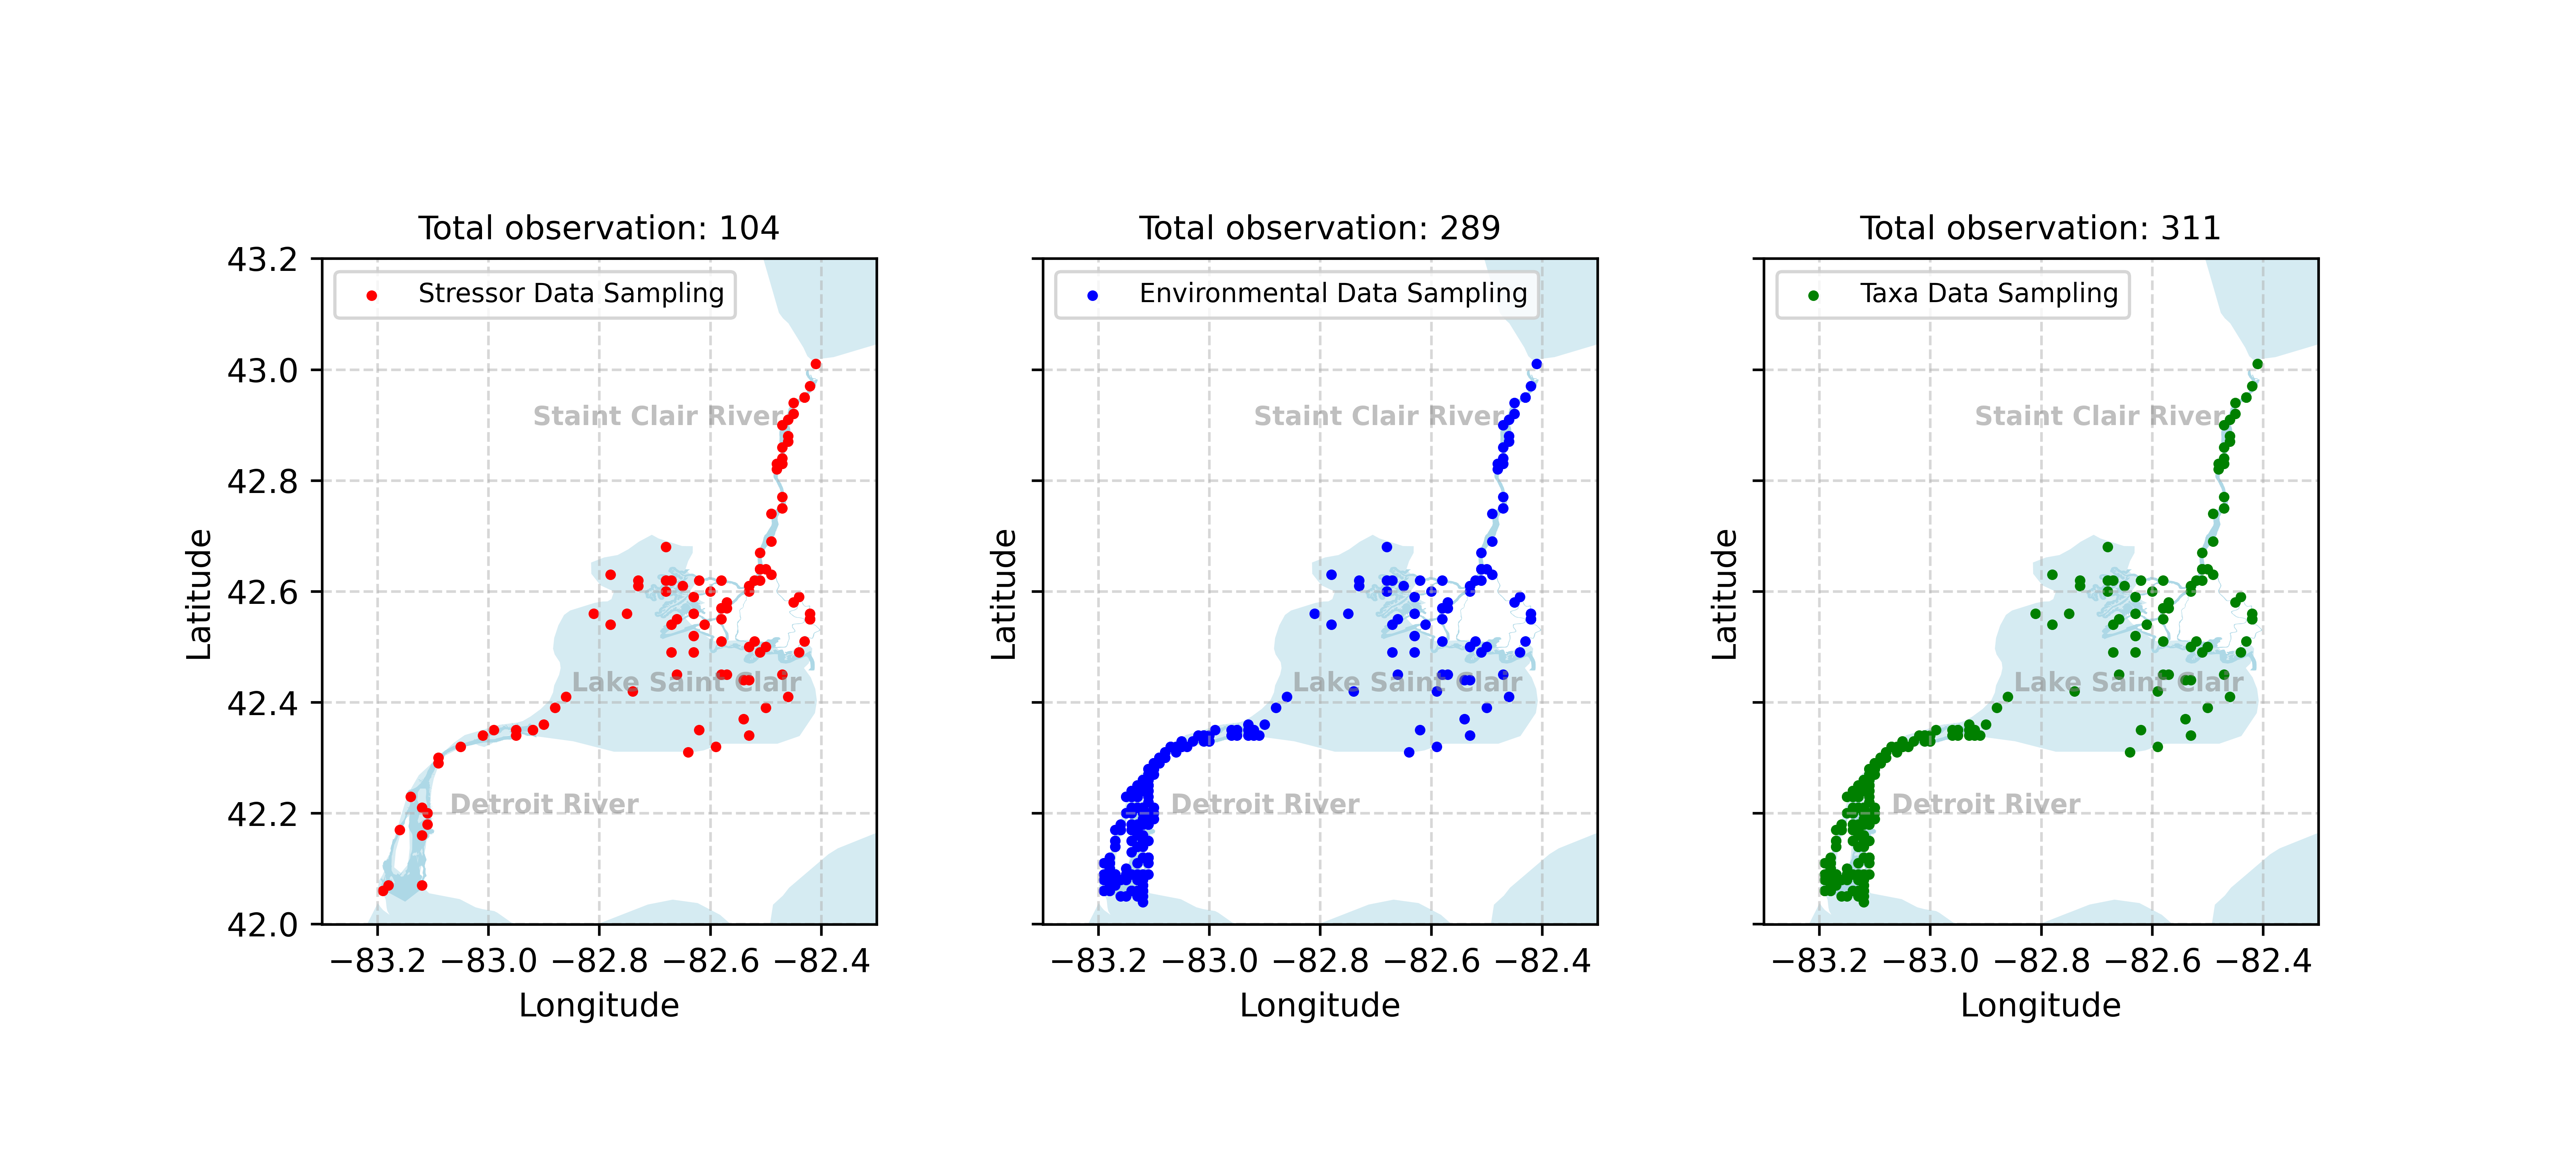
\includegraphics[width=1\textwidth]{../results/different_data_sampling_locations.png}
    \caption{\textit{Map of the SCDRS showing the distribution of locations for which contaminants(left - red points),
environmental covariates (centre - blue points) and zoobenthic data (right - green points) were collected.
Different samples were collected in both temporal and spatial dimensions}}
    \label{fig:different_data_sampling_locations}
\end{figure}

Figure \textcolor{blue}{\ref{fig:different_data_sampling_locations}} shows the numbers
and locations of observations in each dataset.
Note that some locations may be sampled in different
years and only a StationID
\footnote{StationID uniquely identifies a sampling site in both temporal and spatial dimensions.}
(rather than a geographical location) can be
used to confirm the identity of a sampling site.
The three datasets with different types of information (environmental, taxonomic, and stressor) differed in
sample sizes of their observations (row counts).
The stressor dataset contains the fewest observations (104), while the taxonomic and environmental datasets
contain more observations (289 or more).
To prepare a complete dataset for preliminary analysis,
the three datasets were merged by StationID using inner-join operations,
resulting in a comprehensive dataset with 104 observations containing taxonomic, 
environmental, and stressor data across the Lake Huron-Erie Corridor.

This sample size misalignment will be resolved when complete data becomes available in the near future.
Since sample size is the primary difference between current and forthcoming datasets,
the preliminary analysis framework is designed for easy scalability
when additional data becomes available.

\subsection{Large River Case Study: extra water velocity data in Detroit River}
Previous work \cite{Zhang2008} identified limitations in model performance due to insufficient environmental variable coverage.
In a Detroit River-focused analysis \cite{Zhang2008},
a new environmental variable—bottom \textbf{water velocity}—was added,
which was derived by Dr. S. Reitsma using a three-dimensional water flow model.
The focused analysis demonstrated that water velocity is a critical environmental variable for
controlling environmental variation.
Therefore, the Detroit River will serve as a focused study area with water velocity data included,
and it will be conducted once complete stressor data becomes available.

\subsection{Environmental attributes and samples}

Across the three SCDRS surveys, 
location information (longitude and latitude recorded via GPS readings) and 5 environmental attributes
were measured at each sampling site.

\textbf{Temperature ($^\circ$C)} and \textbf{dissolved oxygen concentration ($mg/L$)} were measured using a Hydrolab multimeter. 
\textbf{Water depth ($m$)} was recorded from the Ponar rope.
\textbf{Loss on ignition (\%)} and \textbf{median particle size (phi-units)} were determined during sediment 
processing but are treated as environmental attributes due to their fundamental roles in habitat
characterization (details on their analysis are provided in a later subsection).
% \footnote{Although loss on ignition and median particle size are derived from sediment samples, 
% they are considered environmental variables because they reflect essential physical and chemical habitat features.}
\textbf{Water velocity ($m/s$)} was estimated for the Detroit River area across the three surveys,
displayed in the Table \textcolor{blue}{\ref{tab:environmental_attributes}} along with other cross-corridor attributes.



\begin{table}[htbp]
\centering
\caption{Environmental Attributes}
\label{tab:environmental_attributes}
\begin{tabular}{|>{\centering\arraybackslash}m{4cm}|>{\centering\arraybackslash}m{11cm}|}
\hline
\textbf{Attribute} & \textbf{Ecological Relevance} \\[0.5em]
\hline
Temperature ($^\circ$C) & Controls metabolic rates and organism distribution patterns. \\[0.5em]
\hline
Dissolved Oxygen Concentration ($mg/L$) & Determines survival and excludes oxygen-sensitive taxa when low. \\[0.5em]
\hline
Water Depth ($m$) & Affects light penetration and benthic habitat availability. \\[0.5em]
\hline
Loss on Ignition (\%) & Indicates organic matter content and food availability for benthos. \\[0.5em]
\hline
Median Particle Size (phi-units) & Determines substrate stability and habitat suitability for taxa. \\[0.5em]
\hline
Water Velocity \(^*\) ($m/s$) & Controls flow regime and determines which taxa can colonize sites. \\[0.5em]
\hline
\end{tabular}
\begin{flushleft}
\footnotesize
\textit{(i)} \(^*\) Water velocity was estimated from the model by Dr. S. Reitsma (Detroit River area only, 225 observations) \cite{Zhang2008}.
\\ \textit{(ii)} Other environmental attributes were measured at all sampling sites across the entire survey area (311 observations).
\\ \textit{(iii)} All three surveys (1991, 1999, 2004) followed identical collection protocols and were merged for comprehensive temporal analysis.
\end{flushleft}
\end{table}

These attributes are commonly used to describe baseline environmental conditions in aquatic habitats,
as they are primarily governed by natural physical processes that 
influence taxonomic composition \cite{Davies2006, Turner1989PatternProcess}.

By including these variables as covariates to partially partition the zoobenthic community composition,
we can partially control for natural variation contributed by habitat characteristics, thereby 
isolating the effects of anthropogenic stressors in subsequent analyses 
of community composition patterns.

% However, it is important to note 
% that certain attributes (e.g., organic matter content or temperature) may also be
% indirectly influenced by anthropogenic activities in some settings. 
% Care was taken to interpret their roles in the context of site history and
% land use, but in general, these variables serve as key descriptors of the 
% underlying habitat conditions independent of direct contamination or disturbance.


\subsection{Taxonomic attributes and samples}
The zoobenthos were collected with a Ponar grab sampler. 
After considering the fullness of each grab and the removing of fine materials,
the team applied multiple grabs at each site until a total volume of 2\(L\) sediment was collected.
The sediment samples for organic and metals analysis were preserved in corresponding professional containers, 
all these samples were stored frozen.

One zoobenthic sample replicate from each site was randomly selected and processed, 
while the other two were archived. Samples were sieved into size fractions (4 mm, 1 mm, 0.5 mm, 0.25 mm), 
then elutriated to separate lighter detritus and animals from inorganic sediments. 
Each fraction was sorted under a microscope and organisms were identified to the lowest 
possible taxonomic rank using standard keys. Zoobenthos were preserved in 70\% ethanol in 
labeled vials and archived at the University of Windsor\cite{Zhang2008}.
Immediately after the initial sorting of samples, ten samples were randomly selected to assess the sorting efficiency. 
One sample had a sorting efficiency of 91\%,
while the remaining samples had efficiencies of 96\% or higher.

Specifically, there were 16 taxa recorded from the sediment samples, as shown in the table \textcolor{blue}{\ref{tab:taxonomic_variables}}.
According to their creature characteristics and preferred habitat, 
these taxa can be gently divided into three groups according to their preferred habitat.

\begin{table}[htbp]
\centering
\caption{Benthic Taxa and Preferred Habitat Features}
\label{tab:taxonomic_variables}
\begin{tabular}{|>{\centering\arraybackslash}m{3cm}|>{\centering\arraybackslash}m{5cm}|>{\centering\arraybackslash}m{4cm}|}
\hline
\textbf{Taxa} & \textbf{Explanation} & \textbf{Preferred Habitat} \\
\hline
Nematoda         & Roundworms                   & \multirow{6}{*}{Broad} \\
Chironomidae     & Non-biting midges (larvae)   &  \\
Ceratopogonidae  & Biting midges                &  \\
Amphipoda        & Small crustaceans (scuds)    &  \\
Acari            & Aquatic mites                &  \\
Hydrozoa         & Small predatory animals      &  \\
Gastropoda       & Snails and slugs             &  \\
\hline
Oligochaeta      & Aquatic segmented worms      & \multirow{6}{*}{Depositional zone} \\
Hexagenia        & Mayfly genus (larvae)        &  \\
Dreissena        & Zebra/quagga mussels         &  \\
Hirudinea        & Leeches                      &  \\
Turbellaria      & Flatworms                    &  \\
Sphaeriidae      & Fingernail clams             &  \\
\hline
Caenis           & Mayfly genus (larvae)        & \multirow{3}{*}{Erosional zone} \\
Hydropsychidae   & Net-spinning caddisflies     &  \\
Other Trichoptera& Other caddisfly families     &  \\
\hline
\end{tabular}
\end{table}

\begin{itemize}
    \item \textbf{Broad habitat:} Characterized by a wide range of environmental tolerance. Species in this group can inhabit both depositional and erosional areas, adapting to variable flow velocities, sediment types, and oxygen levels.
    
    \item \textbf{Depositional zone:} Areas with low to moderate water velocity where fine sediments (silt, clay, and organic matter) settle. These habitats often exhibit higher organic content and reduced oxygen penetration, favoring taxa adapted to softer substrates and potentially more enriched nutrient conditions.
    
    \item \textbf{Erosional zone:} Areas with higher flow velocity, coarser substrates (gravel, cobble, or sand), and well-oxygenated water. These habitats support taxa adapted to cling or attach to stable surfaces and withstand stronger currents.
\end{itemize}





\subsection{Stressors attributes and samples}

Sediment samples from each site were thoroughly mixed to ensure homogeneity. The homogenized samples were then split into separate portions for different analyses, including median particle size, total organic carbon (TOC), organic contaminants, and metals.

\begin{itemize}
    \item \textbf{Particle Size:} Median particle size analysis was performed by sieving dried sediment through a series of sieves of decreasing mesh size. Each size fraction was weighed and described using phi units ($\phi = -\log_2 d$), where $d$ is particle size in mm.
    \item \textbf{Total Organic Carbon (TOC):} Sediment TOC(\%OC) was determined using loss on ignition (LOI). Pre-weighed, dried sediment samples were combusted at 450$^\circ$C for 24 hours, and organic carbon was determined gravimetrically by subtracting the remaining mass.
    \item \textbf{Organic Contaminants:} The concentrations of organic contaminants (including 1245-TCB, 1234-TCB, QCB, HCB, OCS, p,p'-DDE, p,p'-DDD, mirex, Heptachlor Epoxide, total PCB)
     were measured using a gas chromatograph equipped with a 63Ni electron capture detector, following standard operating procedures.
    \item \textbf{Metals:} Metal concentrations (including Al, As, Ca, Cd, Co, Cr, Cu, Fe, Mn, Ni, Pb, and Zn) were analyzed using an Inductively Coupled Plasma Optical Emission Spectrophotometer (ICP-OES). For total mercury (Hg), an atomic absorption spectrophotometer (AAS) was used with a vapor generation accessory for increased sensitivity. Liquid samples were introduced into the instrument for metal analysis.
\end{itemize}

\begin{table}[htbp]
\centering
\caption{Sediment Stressors and Classifications}
\label{tab:stressors}

\renewcommand{\arraystretch}{1.2}
\begin{tabular}{|>{\centering\arraybackslash}m{2.5cm}|>{\centering\arraybackslash}m{7cm}|>{\centering\arraybackslash}m{3cm}|}
\hline
\textbf{Variable} & \textbf{Description} & 	\textbf{Type} \\
\hline
\multicolumn{3}{|c|}{\textbf{Metals (mg/kg sediment)}} \\
\hline
Al & Aluminum concentration (nontoxic) & Earth Element \\
Ca & Calcium concentration (nontoxic) & Earth Element \\
Fe & Iron concentration (nontoxic) & Earth Element \\
K & Potassium concentration (nontoxic) & Earth Element \\
Mg & Magnesium concentration (nontoxic) & Earth Element \\
Na & Sodium concentration (nontoxic) & Earth Element \\
As & Arsenic concentration (pollutant) & Trace Metal \\
Bi & Bismuth concentration (pollutant) & Trace Metal \\
Cd & Cadmium concentration (pollutant) & Trace Metal \\
Co & Cobalt concentration (pollutant) & Trace Metal \\
Cr & Chromium concentration (pollutant) & Trace Metal \\
Cu & Copper concentration (pollutant) & Trace Metal \\
Hg & Mercury concentration (highly pollutant) & Trace Metal \\
Mn & Manganese concentration (pollutant) & Trace Metal \\
Ni & Nickel concentration (pollutant) & Trace Metal \\
Pb & Lead concentration (pollutant) & Trace Metal \\
Sb & Antimony concentration (pollutant) & Trace Metal \\
V & Vanadium concentration (pollutant) & Trace Metal \\
Zn & Zinc concentration (pollutant) & Trace Metal \\
\hline
\multicolumn{3}{|c|}{\textbf{Organic Carbon (mg/kg sediment)}} \\
\hline
\%OC & Organic carbon content & Binding agent \\
\hline
\multicolumn{3}{|c|}{\textbf{Organic Contaminants (mg/kg sediment)}} \\
\hline
1245-TCB & 1,2,4,5-Tetrachlorobenzene (hydrocarbon pollutant) & Industrial compound \\
1234-TCB & 1,2,3,4-Tetrachlorobenzene (hydrocarbon pollutant) & Industrial compound \\
QCB & Pentachlorobenzene (hydrocarbon pollutant) & Industrial compound \\
HCB & Hexachlorobenzene (hydrocarbon pollutant) & Industrial compound \\
OCS & Octachlorostyrene (hydrocarbon pollutant) & Industrial compound \\
p,p'-DDE & Dichlorodiphenyldichloroethylene (pesticide) & Organochlorine \\
p,p'-DDD & Dichlorodiphenyldichloroethane (pesticide) & Organochlorine \\
mirex & Mirex (pesticide) & Organochlorine \\
Heptachlor Epoxide & Heptachlor Epoxide (pesticide) & Organochlorine \\
total PCB & Total polychlorinated biphenyls & Sum of all PCBs \\
\hline
\end{tabular}
\end{table}

Quality assurance and chemical analyses were performed in collaboration with the Great Lakes
Institute for Environmental Research (GLIER) at the University of Windsor\cite{Zhang2008}.
Among the chemical variables analyzed, major earth elements (Al, Ca, Fe) are generally non-toxic at typical environmental concentrations, reflecting natural sediment composition. 
However, elevated levels from industrial activities can make them potential stressors, 
leading to difficulties in assessing their impacts due to naturally high background concentrations.

In contrast, trace metals (As, Bi, Cd, Co, Cr, Cu, Hg, Mn, Ni, Pb, Sb, V, Zn) are 
anthropogenic pollutants that bioaccumulate in sediments and cause toxicity in benthic organisms.

Persistent organic pollutants (PCBs, QCB, HCB, OCS, p,p'-DDE, p,p'-DDD, mirex, 
Heptachlor Epoxide) from industrial activities and pesticide use persist in sediments 
and accumulate in food webs, causing chronic effects on aquatic organisms.

Percent organic carbon (\%OC) from decomposed organic matter influences contaminant 
binding and bioavailability, modulating the ecological impact of other pollutants.

By distinguishing between natural major elements (Al, Ca, Fe), trace elements (Co, Mn, Sb, V), 
toxic metals (As, Cd, Cr, Cu, Ni, Pb, Zn), the highly toxic mercury (Hg), organic matter content (\%OC), 
and persistent organic pollutants (including pesticides and industrial compounds), 
these measurements enable a more comprehensive assessment of the sediment stress level and 
its ecological implications for the benthic community.


